% !TEX program = xelatex
% !TEX encoding = UTF-8
%============================================================================
% TrajVis Studio -- User Requirements Specification (Task 2)
% Course : Software Engineering -- 2026 Fall
% Group  : 1  /  Team: 泓泓说的都队
% Author : Chen Hongzhou (Student No. 1240007950), team leader
%
% Structure follows "Task2-User Requirements Specifications Template".docx.
% Every item still to be confirmed is marked \tbd{...} and prints in red.
%============================================================================
\documentclass[12pt,a4paper]{report}

\usepackage{fontspec}
\setmainfont{Times New Roman}
\setsansfont{Helvetica}
\usepackage{xeCJK}
\setCJKmainfont{Songti SC}

\usepackage[a4paper,margin=2.5cm]{geometry}
\usepackage{graphicx}
\usepackage{booktabs}
\usepackage{array}
\usepackage{amsmath,amssymb}
\usepackage{xcolor}
\usepackage{float}
\usepackage{caption}
\usepackage{tikz}
\usetikzlibrary{positioning,arrows.meta,calc,fit,backgrounds}
\usepackage[hidelinks]{hyperref}

% Let long URLs break at slashes instead of running into the margin, and set
% them in the body font rather than the monospace one.
\urlstyle{same}
\makeatletter
\g@addto@macro\UrlBreaks{\do\/\do\-\do\.\do\_\do\:}
\makeatother

% Long identifiers and URLs should break instead of running into the margin.
\emergencystretch=3em

% --- Running header and footer -----------------------------------------
% Every page carries the running title of its chapter at the left of the
% header over a dark rule (the Surface template colours that rule 622423),
% and the page number centred in the footer.
\usepackage{fancyhdr}
% Times New Roman at 12pt needs a taller header box than the 12pt default;
% take the extra height off \topmargin so the text block does not move down.
\setlength{\headheight}{25pt}
\addtolength{\topmargin}{-10pt}
\definecolor{mustrule}{HTML}{622423}
\newcommand{\surfacehead}{%
  \fancyhead[L]{\small\nouppercase{\leftmark}}%
  \fancyfoot[C]{\small\thepage}%
  \renewcommand{\headrulewidth}{1.1pt}%
  \renewcommand{\headrule}{%
    \hbox to\headwidth{\color{mustrule}%
      \leaders\hrule height \headrulewidth\hfill}}%
}
\pagestyle{fancy}
\fancyhf{}
\surfacehead
% Chapter-opening pages use the "plain" style; give it the same furniture.
\fancypagestyle{plain}{\fancyhf{}\surfacehead}
% Header text is "Chapter N <title>", unnumbered front matter just its title.
\def\chaptermark#1{\markboth{Chapter \thechapter\enspace #1}{}}
\def\sectionmark#1{\markright{\thesection\enspace #1}}

% Chapter-based numbering, e.g. "Figure 2-1", "Table 3-2"
\renewcommand{\thefigure}{\thechapter-\arabic{figure}}
\renewcommand{\thetable}{\thechapter-\arabic{table}}

% The template names these two sections "Table of Contents" and "References"
% rather than the class defaults "Contents" and "Bibliography".
\renewcommand{\contentsname}{Table of Contents}
\renewcommand{\bibname}{References}

% Chapter openings carry 50pt above the number, 20pt between the number and
% the title and 40pt below by default.  That suits long chapters; with
% fourteen short ones it leaves the opening page half empty, so the skips are
% roughly halved here.
\makeatletter
\def\@makechapterhead#1{%
  \vspace*{22\p@}%
  {\parindent \z@ \raggedright \normalfont
    \ifnum \c@secnumdepth >\m@ne
      \huge\bfseries \@chapapp\space \thechapter
      \par\nobreak
      \vskip 12\p@
    \fi
    \interlinepenalty\@M
    \Huge \bfseries #1\par\nobreak
    \vskip 26\p@
  }}
\makeatother

% --- Work markers -------------------------------------------------------
% Anything still to be settled prints in red so it cannot ship unnoticed.
% Run `grep -n '\\tbd' report.tex` before submitting; the list must be empty.
\newcommand{\tbd}[1]{{\color{red}\textbf{[TO BE CONFIRMED: #1]}}}
% Compact form for table cells, where the full wording would widen a column.
\newcommand{\tbc}[1]{{\color{red}\textbf{[TBC: #1]}}}
\newcommand{\src}[1]{{\small\itshape (Source: #1)}}

% One block of the nine fields the template prescribes for every functional
% requirement.  These are \section, not \subsection: there is no section
% above them inside the chapter, and a \subsection would number them
% "6.0.1" instead of the template's "6.1".
%
% The skip before and after is tighter than the class default (3.5ex / 2.3ex)
% so that all nine fields of a requirement sit on one page.  With the default
% the last three fields spill onto a second page that is otherwise empty,
% which adds six near-blank pages across Chapters 6--11.
\makeatletter
\newcommand{\reqfield}[2]{%
  % The before-skip is negative on purpose: \@startsection reads its sign to
  % decide whether the paragraph after the heading keeps its first-line
  % indent, and a positive value would indent the field text while every
  % other section does not.
  \@startsection{section}{1}{\z@}%
    {-1.5ex \@plus -.3ex \@minus -.2ex}%
    {0.5ex \@plus .1ex}%
    {\normalfont\Large\bfseries}{#1}#2}
\makeatother

% --- TikZ styles --------------------------------------------------------
\tikzset{
  pbox/.style={rectangle,draw,rounded corners,minimum height=0.78cm,
               align=center,font=\small,thick,inner sep=4pt},
  arr/.style={-{Stealth[length=2.5mm]},thick},
  back/.style={-{Stealth[length=2.5mm]},thick,dashed},
  grp/.style={rectangle,draw,dashed,rounded corners,inner sep=6pt}
}

\begin{document}

%============================================================================
% COVER PAGE
%============================================================================
\begin{titlepage}
  \begin{tikzpicture}[remember picture, overlay]
    \foreach \off in {24, 26.5, 29} {
      \draw[line width=0.6pt]
        ([shift={(\off pt, -\off pt)}]current page.north west)
        rectangle
        ([shift={(-\off pt, \off pt)}]current page.south east);
    }
  \end{tikzpicture}

  \linespread{1.5}\selectfont
  \fontsize{15pt}{18pt}\selectfont
  \centering

  \vspace*{1.2cm}
  
\includegraphics[height=3cm]{logo.jpeg}

  \vspace{2\baselineskip}
  {\bfseries MACAU UNIVERSITY OF SCIENCE AND\\ TECHNOLOGY\par}

  \vspace{\baselineskip}
  {\bfseries School of Computer Science and Engineering\par}
  {\bfseries Faculty of Innovation Engineering\par}

  \vspace{2\baselineskip}
  % The template writes literal "<<" and ">>".  Two adjacent "<" are a T1
  % ligature that renders as the guillemet <<, so put an empty group between
  % them to stop the ligature from forming.
  {\bfseries <{}<{}Software Project for Course Software Engineering>{}>\par}

  \vspace{2\baselineskip}
  \parbox{\textwidth}{\hspace*{1.5cm}%
    \begin{tabular}{@{}l@{: }>{\raggedright\arraybackslash}p{10.5cm}@{}}
      Homework ID  & Task2-User Requirements Specifications \\
      Report Title & TrajVis Studio: User Requirements
                     Specification \\
      Group Number & 1 \\
      Team Members & \begin{tabular}[t]{@{}l@{\hspace{1.2em}}l@{}}
                       Chen Hongzhou & 1240007950 \quad (team leader) \\
                       Zhou Guoxi    & 1240007947 \\
                       Xu Jing       & 1240007919
                     \end{tabular} \\
      Date         & 20 October 2026 \\
    \end{tabular}}
\end{titlepage}

%============================================================================
% FRONT MATTER
%============================================================================
\chapter*{Amendment History}
\markboth{Amendment History}{}

\begin{table}[H]
  \centering
  % Fixed column widths: an "l" column would be widened by whatever the
  % longest cell happens to be, and a "? -> 15cm" marker is long enough to
  % push the table past the 16cm text block.
  \setlength{\tabcolsep}{4.5pt}
  \begin{tabular}{@{}p{1.4cm} p{1.9cm} p{2.7cm} p{3.4cm} >{\raggedright\arraybackslash}p{4.9cm}@{}}
    \toprule[1.5pt]
    \textbf{Version} & \textbf{Date} & \textbf{Modified By} &
      \textbf{Reviewed By} & \textbf{Amendment Details} \\
    \midrule
    1.0 & 2026-10-20 & Chen Hongzhou & Zhou Guoxi, Xu Jing &
      Initial version \\
    \bottomrule[1.5pt]
  \end{tabular}
\end{table}

% The class already sets the running mark for these three lists, so no
% \markboth here: doing it beforehand would leak the next title onto the
% page being closed.
% No \addcontentsline for the contents list itself: the template does not
% list it, and an entry added here would point at the last page of the TOC.
\tableofcontents
\listoffigures
\addcontentsline{toc}{chapter}{List of Figures}
\listoftables
\addcontentsline{toc}{chapter}{List of Tables}

%============================================================================
\chapter{Introduction}
\label{ch:intro}

\section{Purpose}
\label{sec:purpose}

This document is the User Requirements Specification (URS) for
\textbf{TrajVis Studio}, the system proposed for Group~1 in
Task~1. It states what the system must do, from the point of view of the
people who will use it and of the people who will pay for it.

The document serves the build team, two surveyed user representatives and
the course assessors. The assigned customer (the last group on the Part~A
roster) could not be reached after repeated contact; individual members of two
other groups in the class were therefore surveyed as user representatives.
Appendix~A records this limitation and the traceability from each requirement
to its source.

This specification builds on, and does not replace, the project proposal
submitted as Task~1. Where the proposal said what the team intends to
deliver, this document states the requirements in a form that can be
tested one by one.

\section{Notation}
\label{sec:notation}

This specification and its supporting diagrams use the Unified Modelling
Language (UML) notation, as the template requires. In addition:

\begin{itemize}
  \item Every functional requirement carries an identifier \texttt{REQ-x.y}
    and every non-functional requirement an identifier of the form
    \texttt{PERF-x.y}, \texttt{SEC-x.y}, \texttt{AVA-x.y} or
    \texttt{CAP-x.y}.
  \item The word \emph{shall} marks a binding requirement; \emph{should}
    marks a preference that may be traded against cost.
  \item Source identifiers \texttt{S0}--\texttt{S5}, used in Appendix~A,
    name where each requirement came from; \emph{shall} in a table cell is
    binding in the same way as in the running text.
\end{itemize}

\section{Scope}
\label{sec:scope}

\subsection{In scope}
The system accepts a question about recorded movement, written in ordinary
English or Chinese, and returns a finished figure with a plain-language
summary, together with a record that can be re-run. It covers the whole
round trip: understanding the question, retrieving and filtering the
records, choosing and drawing the chart, describing the result, and
measuring its own accuracy.

\subsection{Out of scope}
The system does not collect the movement data, does not clean it, and does
not act as a geographic information system. It does not make planning
decisions; it answers questions about records that already exist. It
offers no mobile application and no public web service.

\section{Context Diagram}
\label{sec:context}

Figure~\ref{fig:context} shows the boundary of the system: what lies inside
it, which outside parties exchange information with it, and what is
exchanged.

\begin{figure}[H]
  \centering
  \resizebox{\textwidth}{!}{%
  \begin{tikzpicture}
    \node[pbox, fill=mustrule!8, minimum width=3.6cm, minimum height=1.7cm]
      (sys) at (0,0)
      {\textbf{TrajVis Studio}\\[2pt]{\scriptsize the system}};

    % One "\\" per node, at the top level of the node text only: TikZ scans
    % for it to split the lines, and a "\\" nested inside a group makes that
    % scan fail.  Long second lines wrap on their own via text width.
    \node[pbox, text width=3.4cm] (analyst) at (-7.0,0)
      {Analyst\\{\scriptsize city planner and transport researcher}};
    \node[pbox, text width=3.8cm] (data) at (6.6,2.0)
      {Trajectory data store\\{\scriptsize records already held}};
    \node[pbox, text width=3.8cm] (bench) at (6.6,-2.0)
      {Recorded benchmark\\{\scriptsize question-and-answer pairs}};
    \node[pbox] (reviewer) at (0,3.0)
      {Reviewer or auditor};

    % Question out, answer back: two parallel arrows so they cannot be read
    % as one line.
    \draw[arr] ([yshift=0.40cm]analyst.east) --
      node[above,font=\scriptsize]{a question} ([yshift=0.40cm]sys.west);
    % Two lines: on one line this label is wider than the gap between the
    % two boxes and would be printed across the Analyst box.
    \draw[arr] ([yshift=-0.40cm]sys.west) --
      node[below,font=\scriptsize,align=center]{a figure, a summary\\and a record}
      ([yshift=-0.40cm]analyst.east);

    \draw[arr] (data) -- node[above,font=\scriptsize,sloped]{records} (sys);
    \draw[arr] (bench) -- node[below,font=\scriptsize,sloped]{test cases} (sys);
    \draw[arr] (reviewer) -- node[right,font=\scriptsize]{a re-run request} (sys);
    \draw[back] (sys) -- node[left,font=\scriptsize]{its measured accuracy}
      (reviewer);
  \end{tikzpicture}}
  \caption{Context diagram: the system and the parties it exchanges
    information with.}
  \label{fig:context}
\end{figure}

\section{Definitions and Acronyms}
\label{sec:definitions}

\begin{table}[H]
  \centering
  \begin{tabular}{@{}l >{\raggedright\arraybackslash}p{11.8cm}@{}}
    \toprule[1.5pt]
    \textbf{Term} & \textbf{Meaning in this document} \\
    \midrule
    Trajectory & The recorded path of one moving object over time, as a
      sequence of timestamped positions. \\
    Analyst & A person who needs an answer about recorded movement but
      cannot write a data query. \\
    Exchange & One question put to the system together with everything the
      system returned for it. \\
    Record & The stored form of an exchange: the question, the request the
      system derived, the data snapshot identifier and the figure. \\
    Benchmark & A published set of recorded question-and-answer pairs used
      to measure the accuracy of the automatic interpretation. \\
    Snapshot & Immutable identifier of the data set an exchange was answered
      from, so that the answer can be reproduced later. \\
    Chart specification & The chart type, fields, filters, scale and time
      zone chosen for a figure. \\
    Confidence notice & The visible statement of how certain the system is
      that it read the question correctly; at low confidence no single
      reading is chosen without the user's confirmation. \\
    URS & User Requirements Specification, this document. \\
    \bottomrule[1.5pt]
  \end{tabular}
\end{table}

\section{References}
\label{sec:references}

\begin{enumerate}
  \item The team's Task~1 submission, \emph{TrajVis Studio: A Self-Service
    Platform for Natural-Language Trajectory Analysis}, Group~1, 2026.
  \item Project repository:
    \url{https://github.com/chenhongzhou666/MUST-SE-TrajVis}
  \item Task~2 description, \emph{User Requirements Specifications},
    Moodle, 2026.09.29.
  \item The template supplied with Task~2,
    \emph{Task2-User Requirements Specifications Template}, Moodle,
    2026.09.29.
\end{enumerate}

The six writing guides listed in Part~D of the task description were read
while preparing this document; they are not cited individually.

\section{Overview}
\label{sec:overview}

Chapter~\ref{ch:general} describes the system and its users in general
terms. Chapter~\ref{ch:constraints} states the software and hardware
constraints and Chapter~\ref{ch:assumptions} the assumptions and
dependencies. Chapter~\ref{ch:master} lists every functional requirement in
summary form and Chapters~\ref{ch:req11}--\ref{ch:req16} define each one in
full. Chapter~\ref{ch:interface} covers the external interfaces and
Chapter~\ref{ch:nfr} the non-functional requirements. Chapter~\ref{ch:domain}
records the requirements that come from the domain rather than from a user.
Appendix~\ref{ch:appendix} records every elicitation source and traces each
requirement back to one.

\section{Contributions}
\label{sec:contributions}

Chen Hongzhou wrote this specification. Zhou Guoxi is the team's contact with
the assigned customer; Xu Jing prepared the questionnaire summarised in
\S\ref{sec:questionnaire} and collected the responses that are cited as
\texttt{S1} and \texttt{S2}. The work after this document will be divided
among the three members along the lines set out in the Task~1 proposal.

%============================================================================
\chapter{General Description}
\label{ch:general}

\section{System Functions}
\label{sec:system-functions}

The system answers questions about recorded movement. A person asks a
question in ordinary language---\emph{which streets stayed busy after nine
in the evening last week}---and receives a figure that answers it, a
sentence saying what the figure shows, and a record of how the answer was
produced.

Its purpose is to remove the queue between the person who has the question
and the person who can query the data. That round trip takes days today and
leaves a picture nobody can check afterwards; the system closes it within
minutes and keeps a record.

At the highest level the system: turns the question into an exact written
request; finds and filters the records the request refers to; chooses and
draws the chart that fits the question; describes the result in one or two
sentences; and measures its own accuracy against a recorded benchmark on
demand.

The functions are enumerated as requirements in
Chapter~\ref{ch:master}. \src{Task~1, \S3.4}

\section{User Characteristics}
\label{sec:user-characteristics}

\begin{table}[H]
  \centering
  \caption{User roles and their characteristics.}
  \label{tab:users}
  \begin{tabular}{@{}p{2.5cm} p{4.3cm} p{2.9cm} p{4.6cm}@{}}
    \toprule[1.5pt]
    \textbf{Role} & \textbf{What they need} & \textbf{Interface type} &
      \textbf{Platform} \\
    \midrule
    Analyst & An answer to a question about movement, without writing a
      query & Self-service, untrained; must work without a manual &
      Desktop web browser \\
    \addlinespace
    Reviewer or auditor & To see how a past answer was produced and to
      re-run it & Trained user; occasional & Desktop web browser \\
    \addlinespace
    Stakeholder & Review the requirements and accept delivery. &
      Documents and review meetings. &
      No runtime role; reads reports only. \\
    \bottomrule[1.5pt]
  \end{tabular}
\end{table}

No role requires installation, a licence key or an account on a third-party
service. Questionnaire respondents used desktop computers (macOS and
Windows); no mobile use was requested.

A ByteDance researcher who works on movement and footprint data has described
this kind of question as a live requirement there; the source is \texttt{S5}
in Appendix~\ref{ch:appendix}, recorded as informal because it came without a
document and supports nothing on its own.

%============================================================================
\chapter{General Constraints}
\label{ch:constraints}

\section{Software Constraints}
\label{sec:software-constraints}

% Tight list spacing: this chapter is only just over one page long, and the
% class default (4pt itemsep) pushes its last bullet onto a page of its own.
\begin{itemize}
  \setlength{\itemsep}{0pt}
  \setlength{\parsep}{0pt}
  \item The system shall be written in Python, because the published method
    it builds on is distributed in Python and re-implementing it in another
    language would discard the working prototype that makes the project
    feasible. \src{Task~1, \S3.8}
  \item The system shall run as a web application and be usable from a
    current desktop browser with no client-side installation.
  \item The system shall reuse existing, openly licensed components rather
    than re-implement them. The parts already identified, with their cost
    and readiness, are listed in Table~\ref{tab:reuse}.
    \src{Task~1, Table~3-3}
  \item The system shall not require any commercial software licence or
    paid cloud service.
\end{itemize}

\begin{table}[H]
  \centering
  \caption{Parts to be reused, with cost and readiness.}
  \label{tab:reuse}
  % Ragged right in the short columns: justified text in a 3 cm column
  % spreads "Public trajectory" across half a line.  \small keeps the table
  % low enough for Chapter 3 to end on one page.
  \small
  \begin{tabular}{@{}>{\raggedright\arraybackslash}p{3.6cm}
                    >{\raggedright\arraybackslash}p{2.2cm}
                    >{\raggedright\arraybackslash}p{2.6cm}
                    >{\raggedright\arraybackslash}p{5.4cm}@{}}
    \toprule[1.5pt]
    \textbf{Part} & \textbf{Licence} & \textbf{Cost} &
      \textbf{Readiness} \\
    \midrule
    Published interpretation method & Open & None &
      Already reproduced by the team, reaching 64\% fully-correct \\
    \addlinespace
    Public trajectory benchmark & Open & None &
      9{,}608 recorded question-and-answer pairs, downloaded and in use \\
    \addlinespace
    Chart rendering library & Open & None &
      Mature; no work required beyond calling it \\
    \addlinespace
    Map and place-name data & Open & None &
      In use for resolving place names written in a question \\
    \bottomrule[1.5pt]
  \end{tabular}
\end{table}

Open-source components only; each licence name is recorded in the project
repository.

\section{Hardware Constraints}
\label{sec:hardware-constraints}

\begin{itemize}
  \setlength{\itemsep}{0pt}
  \setlength{\parsep}{0pt}
  \item The system shall run on an ordinary 24~GB laptop for development and
    single-user demonstration; no server or cloud resource is assumed for
    that environment.
  \item Production multi-user use requires a supported server or
    workstation.
  \item Users shall need no hardware beyond a desktop or laptop computer
    with a pointing device; respondents used macOS and Windows machines and
    asked for nothing more.
\end{itemize}

%============================================================================
\chapter{Assumptions and Dependencies}
\label{ch:assumptions}

\begin{table}[H]
  \centering
  \caption{Assumptions and dependencies, with the consequence if each fails.}
  \label{tab:assumptions}
  \begin{tabular}{@{}p{0.9cm} >{\raggedright\arraybackslash}p{6.4cm} >{\raggedright\arraybackslash}p{6.6cm}@{}}
    \toprule[1.5pt]
    \textbf{Id} & \textbf{Assumption or dependency} &
      \textbf{Consequence if it does not hold} \\
    \midrule
    A1 & The recorded movement data is already held by the customer in a
      usable form. & The project would need a data-preparation stage that
      is not in the plan. \\
    \addlinespace
    A2 & The published benchmark may be used freely and remains available
      at the stated address. & Accuracy could not be measured by the
      system itself and M3 could not be verified. \\
    \addlinespace
    A3 & Analysts are willing to ask questions in ordinary language rather
      than in a query language. & The central feature of the system would
      be unused. \\
    \addlinespace
    A4 & Trajectory source records are de-identified; free-text questions
      may still contain personal data. & A redaction and access-control
      stage would be required before delivery. \\
    \addlinespace
    A5 & The team has continued access to the machines and the network
      used for development. & Development would stop; the plan assumes
      continuous access. \\
    \bottomrule[1.5pt]
  \end{tabular}
\end{table}

%============================================================================
\chapter{Functional Requirements Master List}
\label{ch:master}

This chapter lists the functional requirements in summary form. Each is
defined in full in the chapter named in the last column.

\begin{table}[H]
  \centering
  \caption{Functional requirements master list.}
  \label{tab:master}
  % This table is the widest in the document; a tighter column gap keeps the
  % four columns inside the 16cm text block.
  \setlength{\tabcolsep}{4.5pt}
  \begin{tabular}{@{}l >{\raggedright\arraybackslash}p{3.6cm} >{\raggedright\arraybackslash}p{7.8cm} l@{}}
    \toprule[1.5pt]
    \textbf{Req. ID} & \textbf{Requirement Name} &
      \textbf{Requirement Description} & \textbf{Defined in} \\
    \midrule
    REQ-1.1 & Ask in ordinary language &
      The user states a question in plain English or Chinese and the system
      turns it into an exact written request. & Ch~\ref{ch:req11} \\
    \addlinespace
    REQ-1.2 & Automatic retrieval and filtering &
      The system finds the trajectories the request refers to, resolves
      place names against the records, and returns only the matching
      subset. & Ch~\ref{ch:req12} \\
    \addlinespace
    REQ-1.3 & Automatic chart selection and drawing &
      The system chooses the chart that fits the question and renders the
      figure, with no chart type or plotting tool chosen by the user.
      & Ch~\ref{ch:req13} \\
    \addlinespace
    REQ-1.4 & Plain-language summary of the result &
      The system describes what the figure shows in one or two sentences,
      including the extremes it found. & Ch~\ref{ch:req14} \\
    \addlinespace
    REQ-1.5 & Accuracy dashboard &
      The system re-runs the recorded benchmark on demand, computes its own
      accuracy and shows the result beside its answers. & Ch~\ref{ch:req15} \\
    \addlinespace
    REQ-1.6 & Record and re-run an exchange &
      Every exchange is stored with the question, the derived request, the
      data snapshot identifier and the figure, and can be re-run later to
      reproduce the same figure. & Ch~\ref{ch:req16} \\
    \bottomrule[1.5pt]
  \end{tabular}
\end{table}

The questionnaire responses support the six requirements above; no
additional independent function was requested. Requirements arising later
from the assigned customer or from real potential users will be added to
this list and numbered in sequence.

%============================================================================
% One chapter per functional requirement.  The nine sub-sections inside each
% are the ones the template prescribes; keep their order and their names.
%============================================================================
\chapter{Functional Requirement REQ-1.1}
\label{ch:req11}
\reqfield{Description}{The system shall let a non-specialist ask a
  trajectory question in Chinese or English and see the structured request
  before anything is plotted.}
\reqfield{System Input}{Free text of 1--500 Unicode characters. The question
  may name an object, a place, a time range and a result type. Empty or
  over-length input is rejected.}
\reqfield{Display}{A question box, a waiting indicator and a read-only
  request panel listing the interpreted intent, object, time zone, area,
  chart type and any ambiguity.}
\reqfield{System Processing}{Parse the intent, object, time, place and chart
  fields; resolve relative times and place names; ask for confirmation when
  more than one reading is plausible; execute only after confirmation.}
\reqfield{System Output}{The confirmed request, with intent, time range,
  spatial scope, object filter, chart type, resolved place names, time zone
  and a confidence notice.}
\reqfield{Other}{Source \texttt{S1}/\texttt{S2} Q4, Q9 and Q13: both
  respondents often want to read a pattern they cannot extract themselves,
  both asked to be shown what the system understood and to confirm it before
  anything runs, and both rated support for questions asked in Chinese as
  very important. Feature F1 of the Task~1 proposal.}
\reqfield{Constraints}{The system shall not draw a result from an
  unconfirmed reading, and shall not modify the source records.}
\reqfield{Data Handling}{Store the original question, the normalised
  request, the resolution choices and the confirmation decision. Use UTF-8
  and validate length.}
\reqfield{Error Handling}{If no interpretation is possible, list the missing
  fields and stop. If two readings conflict, ask the user. If the user
  rejects the reading, return to the question.}

\chapter{Functional Requirement REQ-1.2}
\label{ch:req12}
\reqfield{Description}{The system shall retrieve and filter the trajectories
  named in the confirmed request, resolving place names against the
  records.}
\reqfield{System Input}{The confirmed request from REQ-1.1, a selected
  trajectory snapshot and the place-name index. Source data are read-only.}
\reqfield{Display}{A filter summary, progress and a sample table; time, area,
  object and count are listed in the order of the request.}
\reqfield{System Processing}{Apply the time, spatial and object filters,
  resolve place names to identifiers, and keep the snapshot and filter
  settings.}
\reqfield{System Output}{The matching trajectories plus count, time range,
  area, object count, snapshot identifier and any unresolved place names.}
\reqfield{Other}{Source \texttt{S1}/\texttt{S2} Q3 and Q13: both respondents
  work with tabular data, and both rated showing where the data came from as
  important, so a result shall stay inspectable as a table with a stated
  source.}
\reqfield{Constraints}{The system shall not alter source records or silently
  substitute another area, time range or object set.}
\reqfield{Data Handling}{Use UTF-8, an explicit time zone and coordinate
  system; validate dates and coordinates and log the filters with the
  snapshot.}
\reqfield{Error Handling}{If nothing matches, state which filter failed. If a
  place or time is ambiguous, return to REQ-1.1. If data are unavailable,
  report it.}

\chapter{Functional Requirement REQ-1.3}
\label{ch:req13}
\reqfield{Description}{The system shall choose a chart that fits the
  confirmed question and draw it without asking the user to choose a
  plotting tool.}
\reqfield{System Input}{The confirmed request, the matching trajectories, a
  chart category and a display size; the system supports map, line, bar,
  heat map and table.}
\reqfield{Display}{A titled chart with labelled axes or legend, time window,
  units, source label and export controls for PNG, PDF and Excel.}
\reqfield{System Processing}{Use maps for paths, lines for time trends, bars
  for comparisons and heat maps for density; explain any alternative
  chosen.}
\reqfield{System Output}{The rendered figure plus its chart specification,
  time zone, filters and a link to the matching trajectory set.}
\reqfield{Other}{Source \texttt{S1}/\texttt{S2} Q7 and Q8: both respondents
  chose the heat map and the summary, and one of them also chose the map and
  the line chart; in the ranking the summary came first for both and the bar
  chart last or next to last. All five forms are therefore offered. Feature
  F3 of the Task~1 proposal.}
\reqfield{Constraints}{The system shall not truncate an axis without saying
  so, and shall not omit units, source, time window or data label.}
\reqfield{Data Handling}{Store the chart specification with the data
  snapshot; use Unicode labels and consistent time and coordinate formats.}
\reqfield{Error Handling}{If the data cannot support a chart, show the table
  and explain. If rendering fails, keep the data result and report the
  failure.}

\chapter{Functional Requirement REQ-1.4}
\label{ch:req14}
\reqfield{Description}{The system shall describe the figure it has drawn in
  one or two plain-language sentences, including any pattern it can see and
  the largest and smallest values.}
\reqfield{System Input}{The rendered figure, the aggregates behind it, the
  confirmed request and the time, area and object context.}
\reqfield{Display}{The summary beside the figure, with units, time window and
  area stated, and any uncertainty marked.}
\reqfield{System Processing}{State the largest and smallest values, the
  trend, the concentration and the coverage; do not infer causes.}
\reqfield{System Output}{One or two sentences in the language of the
  question.}
\reqfield{Other}{Source \texttt{S1}/\texttt{S2} Q7 and Q8: both respondents
  named the plain-language summary as a wanted output and both ranked it
  first, ahead of every drawn form. Feature F4 of the Task~1 proposal.}
\reqfield{Constraints}{The system shall not state a cause it cannot show, and
  shall not present a low-confidence reading as certain.}
\reqfield{Data Handling}{Generate the summary from the values, never from the
  rendered image, so that the two cannot disagree.}
\reqfield{Error Handling}{If the data are too small or incomplete for a
  summary, say so rather than produce a misleading one.}

\chapter{Functional Requirement REQ-1.5}
\label{ch:req15}
\reqfield{Description}{The system shall measure and display its own accuracy
  on the built-in trajectory benchmark, so that a user can judge how far to
  trust an answer.}
\reqfield{System Input}{The built-in benchmark of 9,608 question--trajectory
  pairs, the version of the system, and a request to run the benchmark now.}
\reqfield{Display}{The accuracy rate, the sample size, the version of the
  system and of the benchmark, the run time and the cases that failed.}
\reqfield{System Processing}{Run the same question-to-trajectory chain used in
  normal operation; count a case as correct only when the whole answer is
  correct.}
\reqfield{System Output}{Numerator, denominator, sample size, benchmark
  version, run timestamp and the list of failed cases.}
\reqfield{Other}{Source \texttt{S1}/\texttt{S2} Q11, Q15 and Q17: both
  respondents asked to see the accuracy rate on the interface, and the errors
  they feared---a wrongly computed time, a misidentified place, a wrong
  value---are exactly the errors such a benchmark exposes. Feature F5 of the
  Task~1 proposal.}
\reqfield{Constraints}{The figure shall not be presented as the accuracy on
  the customer's own questions, and failed cases shall not be hidden.}
\reqfield{Data Handling}{Store the system and benchmark versions, the
  timestamp, the per-case result and the aggregate; keep the data local.}
\reqfield{Error Handling}{If the benchmark is missing or a run fails, report
  the accuracy as unavailable, or as the last successful run with its
  timestamp.}

\chapter{Functional Requirement REQ-1.6}
\label{ch:req16}
\reqfield{Description}{The system shall store every exchange and let the user
  re-run it later, so that a figure can be checked after the fact.}
\reqfield{System Input}{The original question, the confirmed request, the data
  snapshot, the chart specification, the summary, the time zone, the system
  version and the timestamp.}
\reqfield{Display}{A history list, newest first, and a comparison view for a
  re-run.}
\reqfield{System Processing}{Treat the stored exchange as immutable; load its
  snapshot, regenerate the figure and compare the result with the stored
  one.}
\reqfield{System Output}{A re-runnable record, the regenerated figure and a
  pass or fail report on the comparison.}
\reqfield{Other}{Source \texttt{S1}/\texttt{S2} Q10 and Q18: both respondents
  want a result they can keep and check outside the system---a PDF in both
  cases, an image in the earlier format question, and a spreadsheet from one
  of them. Re-running a stored exchange is the team's own proposal
  (\texttt{S4}); the questionnaire did not ask for it. Feature F6 of the
  Task~1 proposal.}
\reqfield{Constraints}{The system shall not overwrite a stored exchange, and
  shall not silently re-run against a newer snapshot.}
\reqfield{Data Handling}{Store records as UTF-8; retain them for two years or
  100,000 exchanges, whichever comes first.}
\reqfield{Error Handling}{If the snapshot is missing, report that the exchange
  cannot be reproduced and name the missing dependency.}

%============================================================================
\chapter{External Interface Requirement}
\label{ch:interface}

\section{Data Interfaces}
\label{sec:data-interfaces}

The system reads recorded movement data from comma-separated (CSV) or Excel
files on the local disk, and reads the benchmark from a file shipped with
the installation. It writes nothing back to either. Column names and the
refresh frequency shall be validated against a sample file supplied with the
data; a file that fails validation is rejected with the failing columns
named.

Results leave the system through an export rather than a write-back: a PNG
image, a PDF or a spreadsheet file. Both respondents asked for a PDF and both
had chosen an image in the earlier format question; one of them also asked
for a spreadsheet (Q10, Q18).

\section{User Interfaces}
\label{sec:user-interfaces}

The system presents a single-page web interface in the user's browser. The
page carries a question box and panels for the interpreted request, the
filters, the figure, the plain-language summary, the accuracy dashboard and
the exchange history with its re-run comparison. A mobile layout is out of
scope: questions are typed on a desktop or laptop with a pointing device.
Both respondents worked that way, one on macOS and one on Windows (Q1, Q2),
and neither asked for a phone or a tablet.

\section{Other Interfaces}
\label{sec:other-interfaces}

There are none. The system uses only the local file system, the browser and
the local CPU and GPU, and opens no network connection of its own.

%============================================================================
\chapter{Non-Functional Requirements}
\label{ch:nfr}

\section{System Performance}
\label{sec:performance}

\begin{table}[H]
  \centering
  \caption{Performance requirements.}
  \label{tab:perf}
  \setlength{\tabcolsep}{4.5pt}
  \begin{tabular}{@{}l >{\raggedright\arraybackslash}p{9.4cm} l@{}}
    \toprule[1.5pt]
    \textbf{Req. Id} & \textbf{Description} & \textbf{Response time} \\
    \midrule
    PERF-1.1 & Time from asking a question to receiving the figure and the
      summary, for a single question. & 10--30\,s; max 60\,s \\
    \addlinespace
    PERF-1.2 & Time to narrow a result already on screen---adding a filter
      or changing the time window---and see the figure redrawn.
      & Under 10 seconds \\
    \addlinespace
    PERF-1.3 & Time to re-run one recorded exchange and rebuild the same
      figure from the record alone. & Under 30 seconds \\
    \addlinespace
    PERF-1.4 & Time to re-run the whole recorded benchmark and report a new
      accuracy figure; a batch job, not an interactive one. & Under 24 hours \\
    \bottomrule[1.5pt]
  \end{tabular}
\end{table}

PERF-1.1 is the project's headline commitment, carried over from Task~1
measure~M1. Asked how long they would wait for one answer (Q14), one
respondent accepted 30\,s to one minute and the other 10--30\,s; the target
band takes the tighter answer and the 60\,s maximum takes the looser one. The
figures are measured on the reference laptop (24\,GB of memory, 10\,GB of
data, one user, warm start). They were put to the respondents as a team
proposal rather than set by the customer; Appendix~A records this.

\section{Information Security}
\label{sec:security}

\begin{table}[H]
  \centering
  \caption{Information security requirements.}
  \label{tab:security}
  \begin{tabular}{@{}l >{\raggedright\arraybackslash}p{13.0cm}@{}}
    \toprule[1.5pt]
    \textbf{Req. Id} & \textbf{Description} \\
    \midrule
    SEC-1.1 & Credentials and any personal data shall not be transmitted in
      plain text over any network. \\
    \addlinespace
    SEC-1.2 & Any personal data shall be held only in an environment that
      has passed full system testing; it shall not be held in a development
      or demonstration environment. \\
    \addlinespace
    SEC-1.3 & The system shall meet the information security policies of
      Macau University of Science and Technology and of the assigned
      customer. The customer has not named the policy documents; the team
      applies the University's general rules in the meantime. \\
    \addlinespace
    SEC-1.4 & The system shall not hold data that could identify an
      individual, and shall not transmit records to any third-party service
      without the customer's written agreement. \\
    \bottomrule[1.5pt]
  \end{tabular}
\end{table}

SEC-1.3 cites no document that the team has not read. Q19 records only that
both respondents had heard of data-use rules; neither was asked to name one,
and the assigned customer named none.

\section{Availability and Retention}
\label{sec:availability}

\begin{table}[H]
  \centering
  \caption{Availability requirements.}
  \label{tab:availability}
  \begin{tabular}{@{}l >{\raggedright\arraybackslash}p{13.0cm}@{}}
    \toprule[1.5pt]
    \textbf{Req. Id} & \textbf{Description} \\
    \midrule
    AVA-1.1 & The system shall be available during the customer's working
      hours, 09:00--18:00, on working days. \\
    \addlinespace
    AVA-1.2 & Planned unavailability shall not exceed one working day per
      calendar month and shall be announced at least 24 hours in advance. \\
    \addlinespace
    AVA-1.3 & Unplanned unavailability shall not exceed four hours per
      calendar month. \\
    \addlinespace
    AVA-1.4 & A recorded exchange shall remain re-runnable for at least two
      years after it was made. \\
    \bottomrule[1.5pt]
  \end{tabular}
\end{table}

\section{Capacity}
\label{sec:capacity}

\begin{table}[H]
  \centering
  \caption{Capacity requirements.}
  \label{tab:capacity}
  \begin{tabular}{@{}l >{\raggedright\arraybackslash}p{11.0cm} l@{}}
    \toprule[1.5pt]
    \textbf{Req. Id} & \textbf{Description} & \textbf{Value} \\
    \midrule
    CAP-1.1 & Volume of recorded movement data the system must hold and
      query in year ONE. & 10\,GB \\
    \addlinespace
    CAP-1.2 & The same for year TWO. & 30\,GB \\
    \addlinespace
    CAP-1.3 & The same for year THREE. & 60\,GB \\
    \addlinespace
    CAP-2.1 & Concurrent users the system must serve in year ONE. & 5 \\
    \addlinespace
    CAP-2.2 & The same for year TWO. & 10 \\
    \addlinespace
    CAP-2.3 & The same for year THREE. & 20 \\
    \addlinespace
    CAP-3.1 & Number of exchanges that must remain stored and re-runnable.
      & 100,000 \\
    \bottomrule[1.5pt]
  \end{tabular}
\end{table}

The values form a planning envelope, not a commitment the customer set. The
questionnaire does not ask about data volume or concurrent users, and the
closing invitation to raise anything the questions had missed (Q20) produced
no answer from either respondent, so the envelope rests on \texttt{S4} alone.
Sources: \texttt{S3} and \texttt{S4}.

%============================================================================
% The task description asks for domain requirements as well as functional
% and non-functional ones, but the template has no section for them.  This
% chapter fills that gap; delete it only if the assessor confirms otherwise.
%============================================================================
\chapter{Domain Requirements}
\label{ch:domain}

The task description asks that the specification cover functional,
non-functional \emph{and} domain requirements. The supplied template has no
section for the third kind, so they are recorded here.

\begin{table}[H]
  \centering
  \caption{Requirements arising from the domain rather than from a user.}
  \label{tab:domain}
  \begin{tabular}{@{}l >{\raggedright\arraybackslash}p{13.0cm}@{}}
    \toprule[1.5pt]
    \textbf{Req. Id} & \textbf{Description} \\
    \midrule
    DOM-1.1 & Time shall be handled with an explicit time zone; a question
      naming a time of day shall be interpreted in the time zone of the
      records, not of the person asking. \\
    \addlinespace
    DOM-1.2 & Positions shall be handled in a stated coordinate system, and
      distances shall be computed on the sphere rather than on a flat map. \\
    \addlinespace
    DOM-1.3 & A place name in a question shall be resolved against the
      names as they appear in the records, and the resolution used shall be
      shown to the user. \\
    \addlinespace
    DOM-1.4 & Charts shall follow the conventions of the domain: a stated
      and labelled scale, a stated time window, and no truncation of an
      axis without saying so. \src{Task~1, \S3.5 measure M4} \\
    \addlinespace
    DOM-1.5 & The system shall comply with the Macau Personal Data
      Protection Act (Law No.~8/2005) and with the licence that governs the
      map data it uses. Both respondents had heard of rules covering privacy,
      mapping and cross-border transfer (Q19), but the questionnaire did not
      ask them to name a document, so the Act is taken from published law
      rather than from the customer; see Appendix~A. \\
    \bottomrule[1.5pt]
  \end{tabular}
\end{table}

%============================================================================
% Part A asks for three elicitation sources and makes the assigned customer
% compulsory.  This appendix records what was actually obtained, so that the
% gap is visible rather than papered over.
%============================================================================
\appendix
% \thechapter is \Alph{chapter} after \appendix, so the running header would
% otherwise read "Chapter A".  Say "Appendix" instead.
\def\chaptermark#1{\markboth{Appendix \thechapter\enspace #1}{}}

\chapter{Source Register and Traceability}
\label{ch:appendix}

Part~A of the task asks that the requirements be elicited from three kinds of
source: the assigned customer, which is compulsory; real potential users; and
members of the team. This appendix records which sources were actually used,
what each one supplied, and where the record falls short.

\section{Register of Elicitation Sources}
\label{sec:sources}

\begin{table}[H]
  \centering
  \caption{Every source cited in this document, and how it was obtained.}
  \label{tab:sources}
  \setlength{\tabcolsep}{4.5pt}
  \begin{tabular}{@{}l >{\raggedright\arraybackslash}p{3.9cm}
                    >{\raggedright\arraybackslash}p{4.5cm}
                    >{\raggedright\arraybackslash}p{2.6cm} l@{}}
    \toprule[1.5pt]
    \textbf{Id} & \textbf{Source} & \textbf{Method} & \textbf{Date} &
      \textbf{Status} \\
    \midrule
    S0 & Assigned customer: the last group on the Part~A roster, which is
      Group~1's customer under the roster rule & Contacted through the course
      group, more than once, and not reached
      & before 19 Oct 2026 & Not obtained \\
    \addlinespace
    S1 & User representative R1, a member of another group in the class &
      Written questionnaire of 20 questions, returned as a platform export &
      19 Oct 2026, 11:36 & Received \\
    \addlinespace
    S2 & User representative R2, a member of a further group in the class &
      The same instrument, returned as a platform export &
      20 Oct 2026, 09:22 & Received \\
    \addlinespace
    S3 & The team's Task~1 proposal & Written by the team &
      7 Oct 2026 & Used \\
    \addlinespace
    S4 & Team planning assumptions about scale and availability & Written
      by the team & 20 Oct 2026 & Provisional \\
    \addlinespace
    S5 & Professional user: a researcher at ByteDance working on movement
      and footprint data & Reported to the team by Chen Hongzhou; no document
      supplied & 20 Oct 2026 & Informal \\
    \bottomrule[1.5pt]
  \end{tabular}
\end{table}

\texttt{S5} is the weakest entry in the register and is marked as such. It
records that a researcher at ByteDance who works on movement and footprint
data described analysis of this kind as a live requirement in that
organisation; it was passed on verbally and no document was supplied. Nothing
in Chapters~\ref{ch:general}--\ref{ch:domain} is justified by \texttt{S5}
alone. It is recorded because it shows that the need is not confined to the
two respondents, and because omitting it would make the account of what was
gathered less complete than it is.

\section{Status of the Assigned Customer}
\label{sec:assigned-customer}

The roster rule makes the last team on the Part~A roster the customer of the
first team, so Group~1's assigned customer is the last group. That group was
contacted through the course group more than once before 19 October 2026 and
could not be reached.

Because the assigned customer could not be reached, the questionnaire was put
instead to individual members of other groups in the class: R1 from one group
and R2 from another. They answered as ordinary users of the system, not as a
team and not as the customer.

The team has not presented a user representative as the assigned customer.
Where a requirement rests on S0, the table in \S\ref{sec:traceability} says so
and the requirement itself carries a visible marker. The obligation is
therefore unmet rather than concealed.

\section{Summary of the Questionnaire}
\label{sec:questionnaire}

One instrument was used for both respondents: a written questionnaire of
twenty questions, sent through the course group and answered in the
respondent's own time; the platform recorded the submission time shown in
Table~\ref{tab:sources}. The first six questions establish the context of the
respondent---operating system, device, the kind of data handled, whether they
often want to read a pattern they cannot extract themselves, how they analyse
data today, and which step they find hardest. Q7 and Q8 ask what form the
answer should take, first by multiple choice and then by ranking. Q9 asks
what the system should do when it has misread the question. Q10 and Q18 ask
what the result must be exportable as. Q11 asks how much accuracy matters and
Q13 rates five properties of the tool on a five-point scale. Q14 sets the
acceptable waiting time and Q15 the errors the respondent fears. Q12 is a
control question that instructs the respondent to pick a given option; both
answered it correctly, so neither response was discarded as careless. Q16
invites a recent worked example, Q17 asks whether the accuracy rate should be
shown, Q19 asks whether the respondent has heard of data-use rules, and Q20
is an open invitation to name anything the questions missed.

Two answers carry more weight than the rest. Q8 ranked the one-sentence
summary first for both respondents, ahead of every drawn form, which is why
the summary is a requirement of its own (Chapter~\ref{ch:master}) rather than a
caption on a figure. Q9 was answered identically by both---show me what you
understood and ask me to confirm---which is why REQ-1.1 stops for
confirmation instead of plotting from its best guess.

Some questions produced nothing usable, and are recorded as such. Neither
respondent could give a worked example when Q16 asked for one, and neither
named an unforeseen constraint in Q20; none has been invented here. Q11 split,
one respondent rating accuracy as very important and the other as neither
important nor unimportant, but both then asked in Q17 to see the accuracy
rate on the interface, and REQ-1.5 follows Q17. Neither respondent named a
policy document, because Q19 did not ask for one.

\section{Traceability Matrix}
\label{sec:traceability}

\begin{table}[H]
  \centering
  \caption{Each requirement against the source that supports it.}
  \label{tab:trace}
  % \small stays inside the float, which is a group of its own, so nothing
  % leaks into the body text after the table.
  \small
  \setlength{\tabcolsep}{4.5pt}
  \begin{tabular}{@{}l >{\raggedright\arraybackslash}p{5.0cm}
                    >{\raggedright\arraybackslash}p{8.2cm}@{}}
    \toprule[1.5pt]
    \textbf{Requirement} & \textbf{Source} & \textbf{Support} \\
    \midrule
    REQ-1.1 & S1, S2 (Q4, Q9, Q13); S3 & Questions from people who cannot
      write a query; the reading shown and confirmed before it runs \\
    \addlinespace
    REQ-1.2 & S1, S2 (Q3, Q13); S3 & Tabular data; the result stays
      inspectable as a table with a stated source \\
    \addlinespace
    REQ-1.3 & S1, S2 (Q7--Q8); S3 & Heat map and summary chosen by both; map
      and line by one; all five forms ranked \\
    \addlinespace
    REQ-1.4 & S1, S2 (Q7, Q8); S3 & The plain-language summary ranked first by
      both respondents \\
    \addlinespace
    REQ-1.5 & S1, S2 (Q11, Q15, Q17); S3 & Accuracy requested on the
      interface; time, place and value named as the feared errors \\
    \addlinespace
    REQ-1.6 & S4; S1, S2 (Q10, Q18) & Team proposal; respondents want the
      result kept and checked outside the system \\
    \addlinespace
    PERF-1.1 & S4; S3 (measure M1); S1, S2 (Q14) & Waiting time asked for;
      band and ceiling set by the team \\
    \addlinespace
    SEC-1.3 & S0 (open); S1, S2 (Q19) & No policy document named; the
      University's general rules apply \\
    \addlinespace
    AVA-1.1--1.4 & S4 & Working hours and allowance proposed by the team \\
    \addlinespace
    CAP-1.1--3.1 & S4 & Envelope proposed by the team; not put to the
      respondents \\
    \addlinespace
    DOM-1.5 & S0 (open); S1, S2 (Q19) & Statutory duty taken from published
      law, not from the customer \\
    \bottomrule[1.5pt]
  \end{tabular}
\end{table}

\section{Confirmation and Limitations}
\label{sec:limitations}

The requirements in this document have not been confirmed by the assigned
customer. They rest on S1, S2, S3 and S4, and five limits follow.

\begin{enumerate}
  \item Part~A source~1 is not satisfied. S0 is recorded as not obtained;
    the gap is stated here and in \S\ref{sec:purpose} rather than hidden.
  \item The non-functional numbers are a team proposal, not values the
    customer set. Only the waiting time was put to the respondents in a form
    they could answer (Q14), and where the two answers differed the tighter
    one was taken as the target. The data volumes and the concurrent-user
    figures were never put to them, and Q20 produced no comment on them.
  \item The institution's software and licence policy was not available by
    name. SEC-1.3 records that the University's general rules apply in the
    meantime, and no document is cited that the team has not read.
  \item Both respondents answered as ordinary users rather than as transport
    or planning specialists, and neither could offer a worked example when
    asked for one (Q16). The domain requirements of Chapter~\ref{ch:domain}
    therefore rest on published practice rather than on an expert interview.
  \item \texttt{S5} is informal. It shows that a professional user in
    industry wants this capability, but it came without a document, carries
    no figure and supports no individual requirement; no requirement in this
    document would fall if \texttt{S5} were withdrawn.
\end{enumerate}

If the assigned customer replies before submission, S0 will be recorded as
received, the requirements it touches will be re-checked against the reply,
and this appendix revised before the report is handed in.

%============================================================================
% \begin{thebibliography} is itself a \chapter*, so the \addcontentsline
% must sit inside it; placed outside, the contents entry would take the
% page number of the previous chapter's last page.
%============================================================================
\begin{thebibliography}{9}
\addcontentsline{toc}{chapter}{References}
\markboth{References}{}

\bibitem{task1} Group~1, \emph{TrajVis Studio: A Self-Service Platform for
  Natural-Language Trajectory Analysis}, Task~1 project proposal, Software
  Engineering, MUST, 2026.

\bibitem{task2} \emph{User Requirements Specifications Description},
  Software Engineering, MUST, 2026.09.29.

\bibitem{template} \emph{Task2-User Requirements Specifications Template},
  Software Engineering, MUST, 2026.09.29.

\bibitem{repo} Project repository,
  \url{https://github.com/chenhongzhou666/MUST-SE-TrajVis}

\bibitem{acl} V.~J.~Wei et al., \emph{Text-to-TrajVis}, Findings of ACL,
  2026. \url{https://aclanthology.org/2026.findings-acl.972/}

\end{thebibliography}

\end{document}
